


\section{Q2}
\label{part2}
\begin{enumerate}

\item Ingest the 100 URIs from their resulting WARC files into a SOLR instance
	- see the code + tutorial at: https://github.com/ukwa/webarchive-discovery 

\item Demonstrate several functioning queries on the files (a full front-end is not required)
	- describe the configuration choices you made in setting up SOLR and processing the documents

\end{enumerate}

\subsection{Description}
\begin{enumerate}

\item I configured a local SOLR instance and indexed 100 WARC files in it.

\item I used default configurations for SOLR.

\item I performed various queries on SOLR and included the resulting screenshots in this report.

\end{enumerate}

\newpage


\subsubsection{Functioning queries on SOLR}


\begin{figure}[ht]    
    \begin{center}
        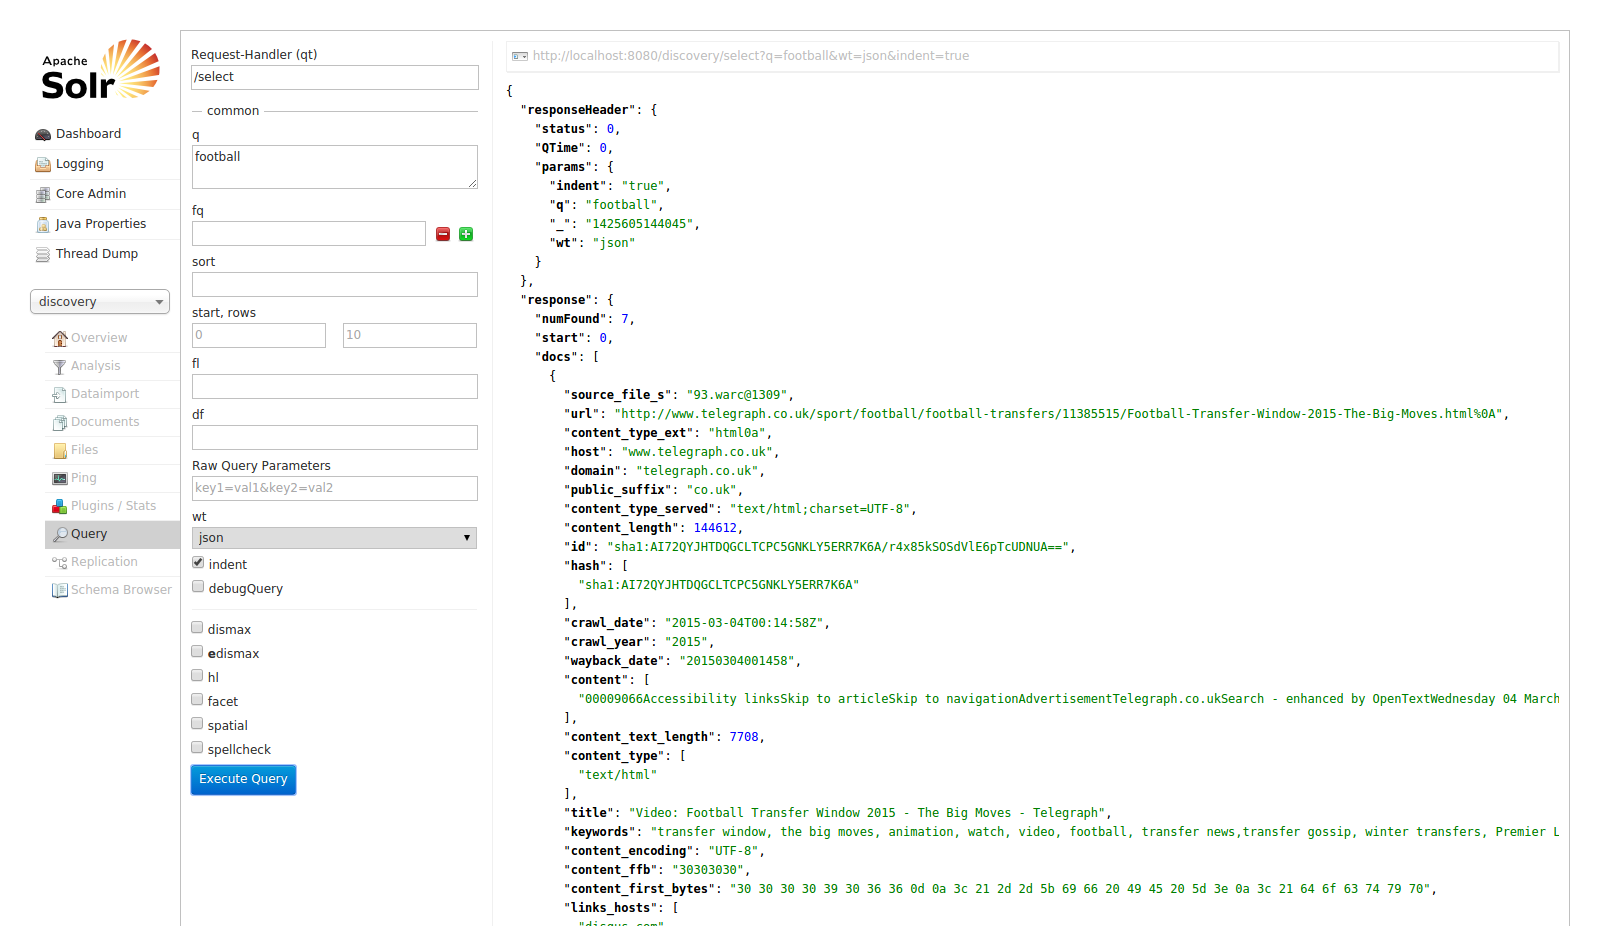
\includegraphics[width=\paperwidth]{query1.png}
        \caption{Search for 'football'}        
    \end{center}
\end{figure}

\begin{figure}[ht]    
    \begin{center}
        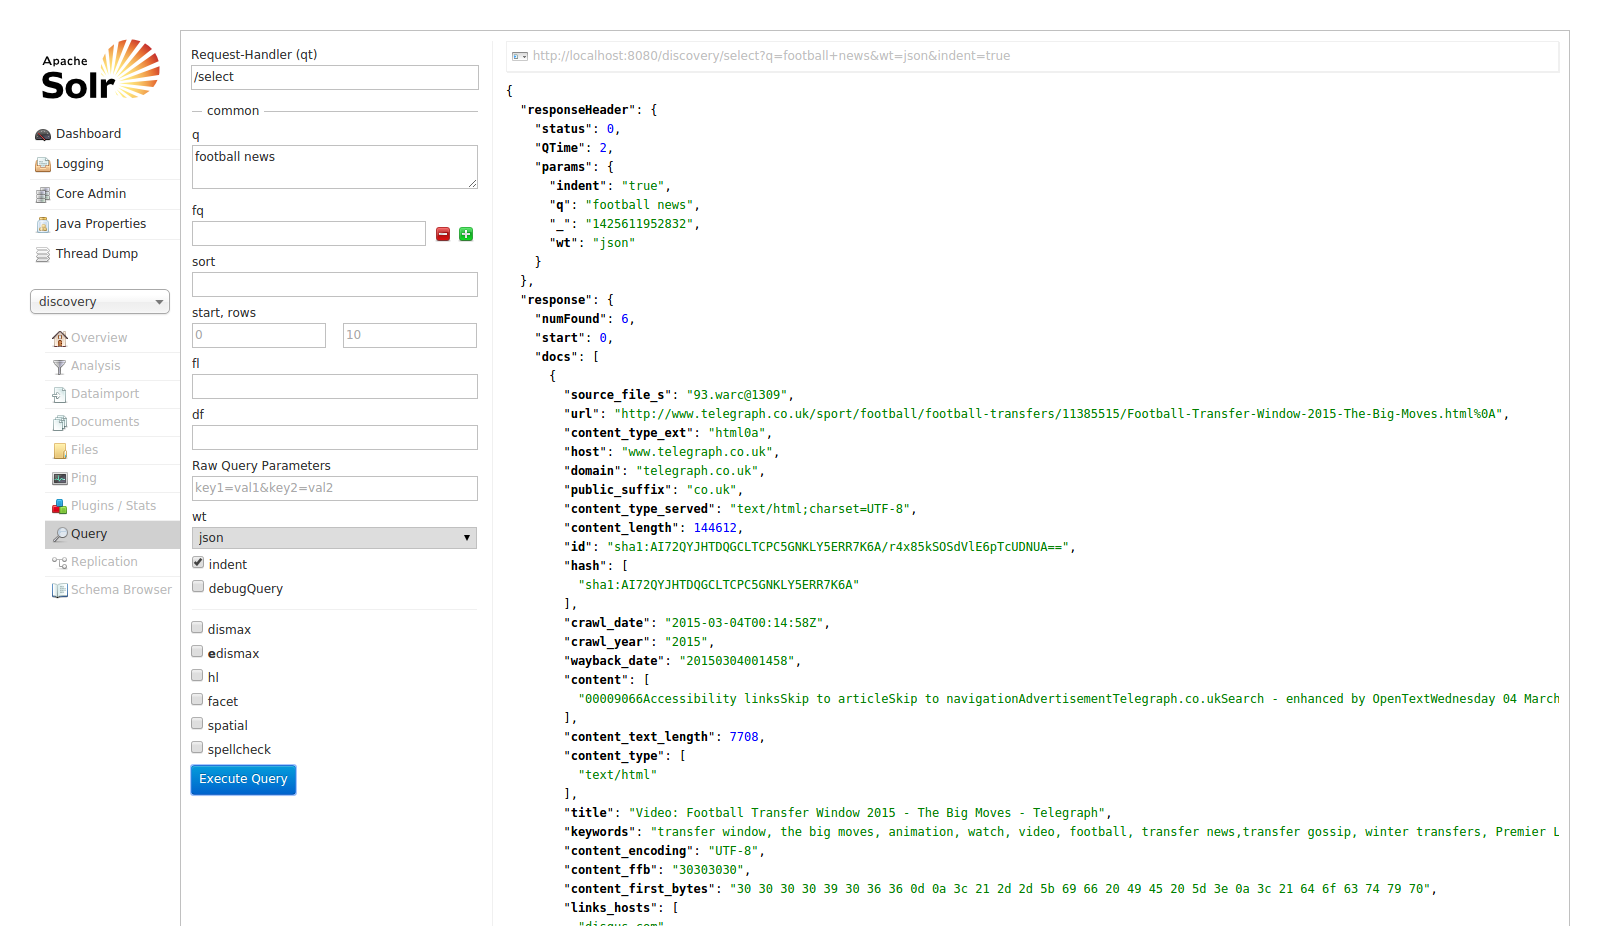
\includegraphics[width=\paperwidth]{query2.png}
        \caption{Search for 'football news'}
    \end{center}
\end{figure}

\begin{figure}[ht]    
    \begin{center}
        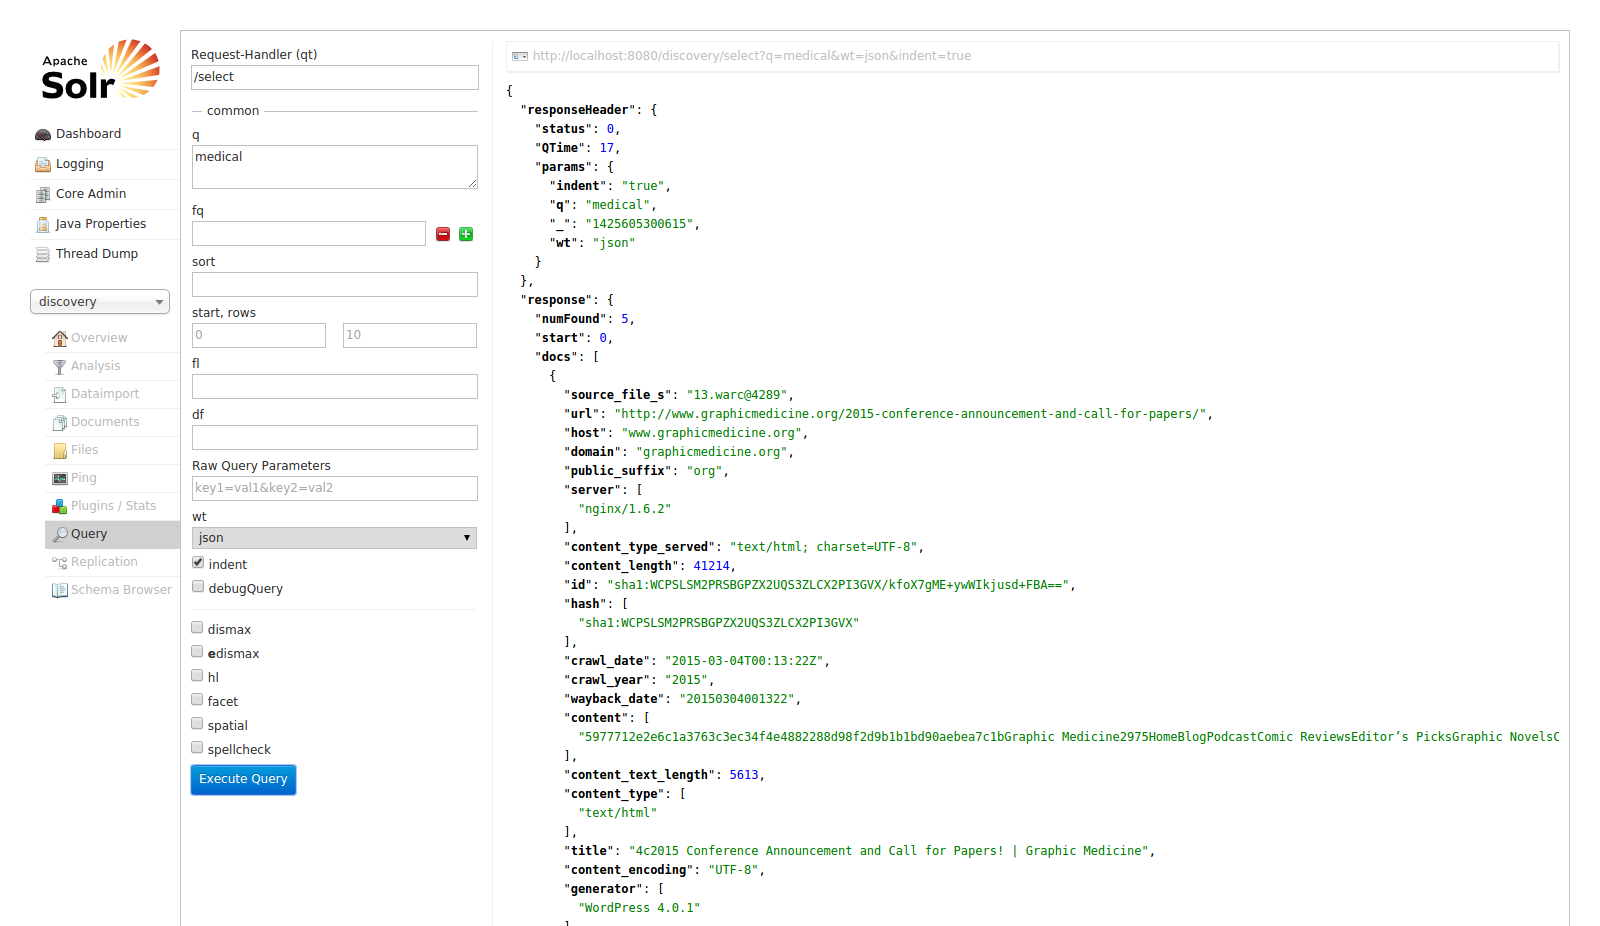
\includegraphics[width=\paperwidth]{query3.png}
        \caption{Search for 'medical'}
    \end{center}
\end{figure}

\begin{figure}[ht]    
    \begin{center}
        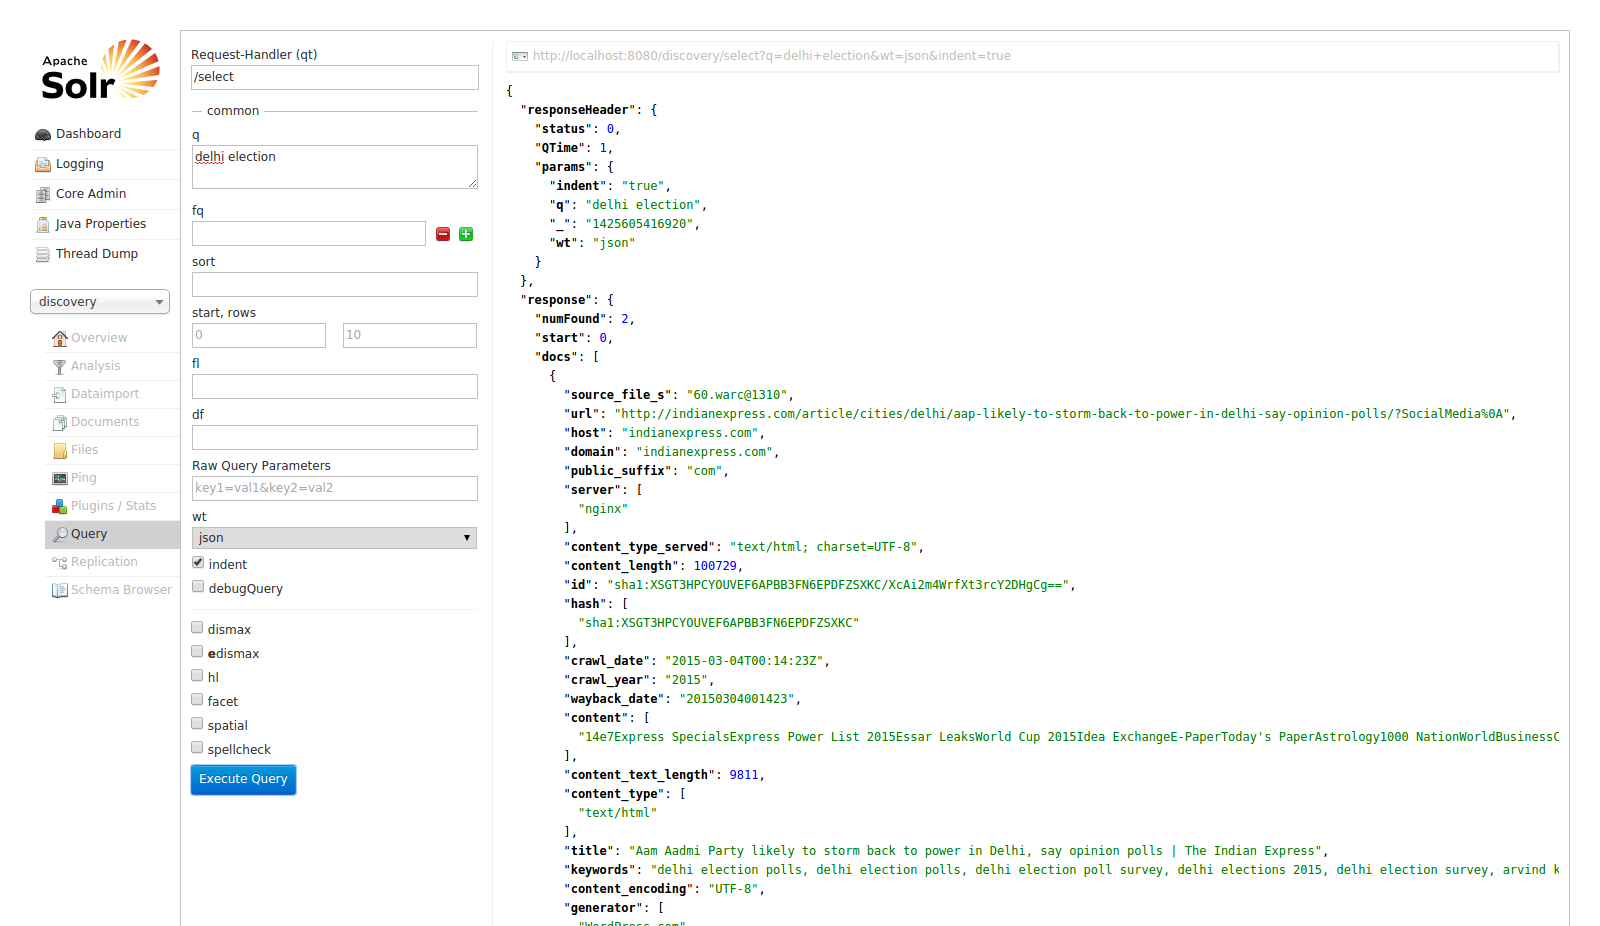
\includegraphics[width=\paperwidth]{query4.png}
        \caption{Search for 'delhi election'}
    \end{center}
\end{figure}

\begin{figure}[ht]    
    \begin{center}
        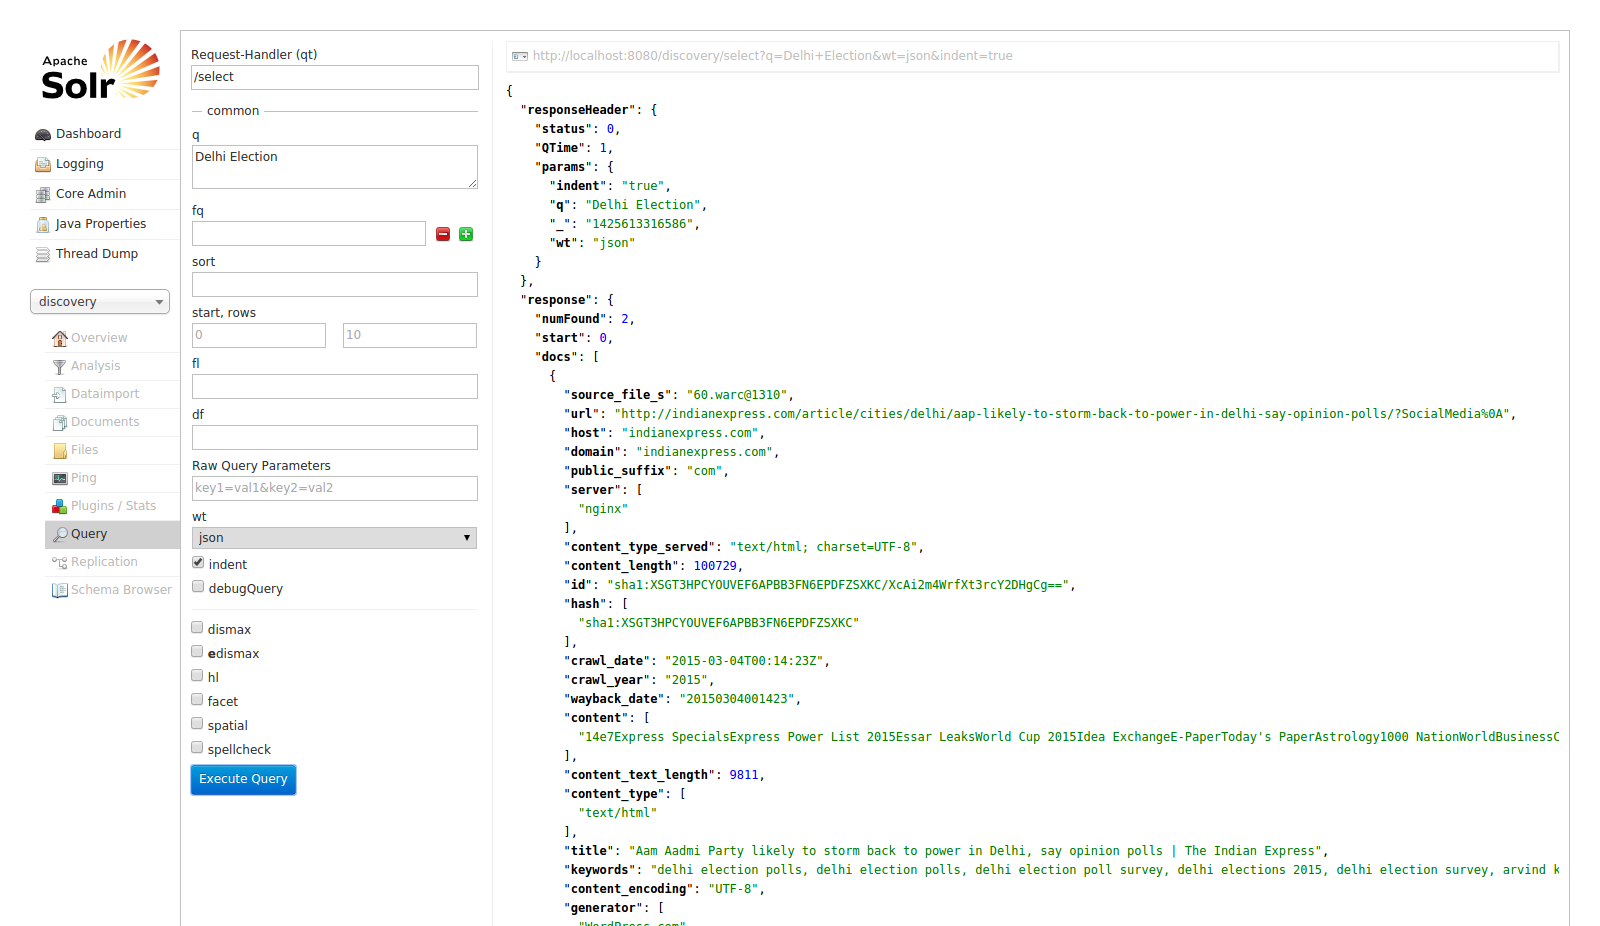
\includegraphics[width=\paperwidth]{query5.png}
        \caption{Search for 'Delhi Election' using different case than previous query}
    \end{center}
\end{figure}

\begin{figure}[ht]    
    \begin{center}
        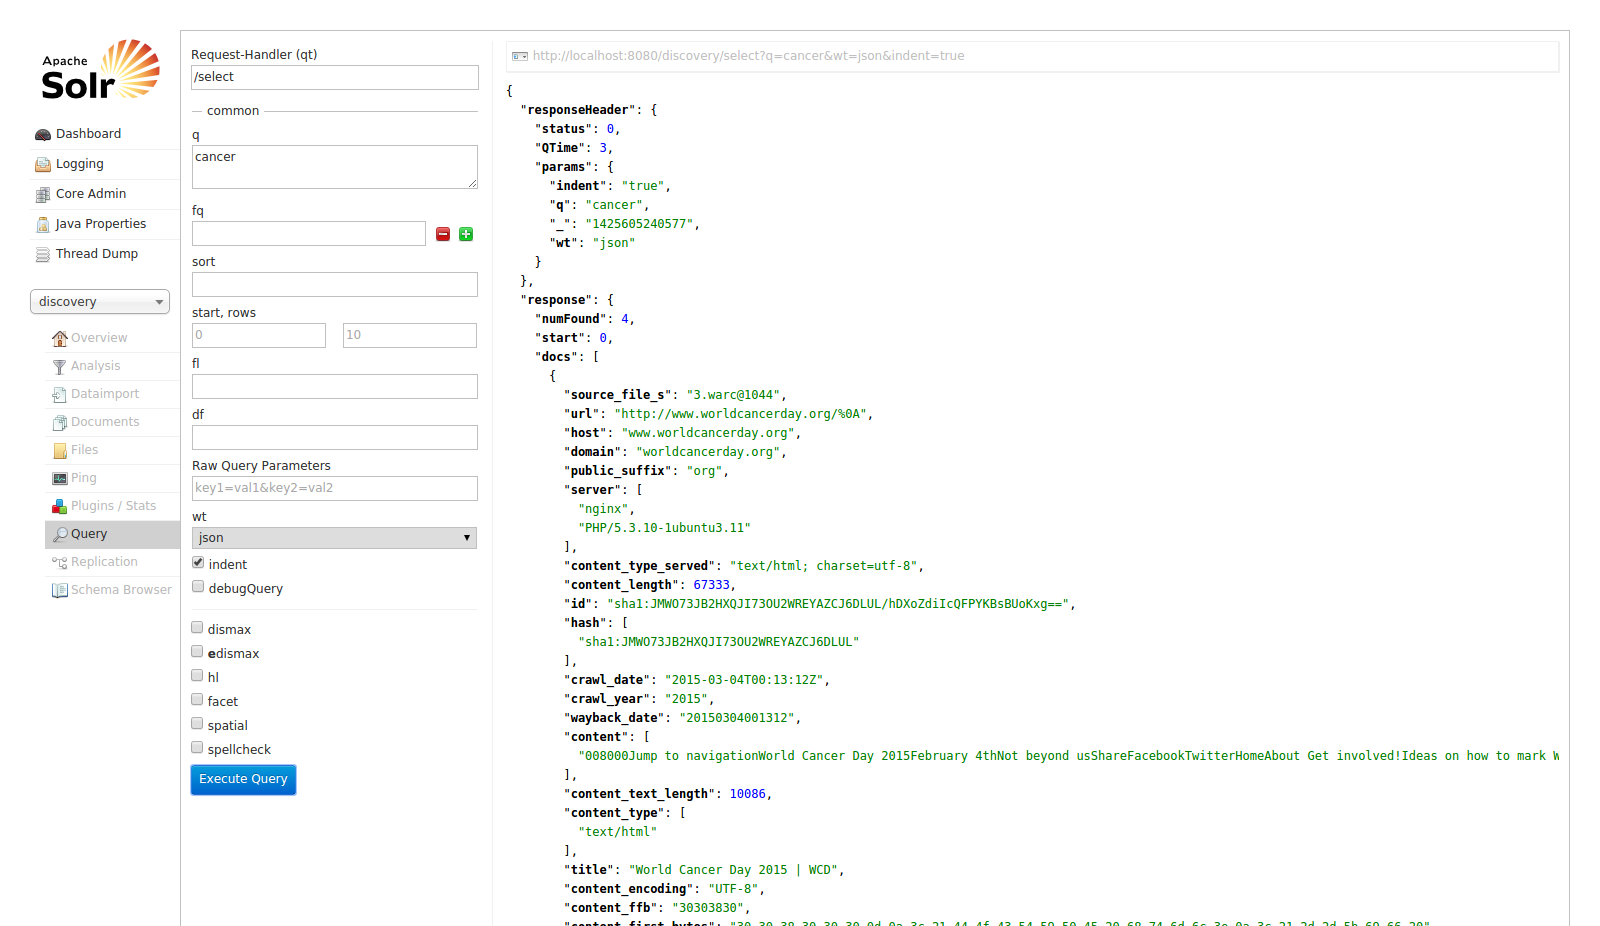
\includegraphics[width=\paperwidth]{query6.png}
        \caption{Search for 'cancer'}
    \end{center}
\end{figure}
